%% The first command in your LaTeX source must be the \documentclass command.
%%
%% Options:
%% twocolumn : Two column layout.
%% hf: enable header and footer.
\documentclass[
twocolumn,
% hf,
]{ceurart}

\usepackage[T1]{fontenc}
\usepackage{lmodern}

% Ismael - Las urls de la bibliografía se salen de la bounding box, esto lo arregla
\usepackage{xurl}
\usepackage{hyperref}
% Fin Ismael

%%
%% One can fix some overfulls
\sloppy

%%
%% Minted listings support 
%% Need pygment <http://pygments.org/> <http://pypi.python.org/pypi/Pygments>
%\usepackage{minted}
%% auto break lines
%\setminted{breaklines=true}

%%
%% end of the preamble, start of the body of the document source.
\begin{document}

%%
%% Rights management information.
%% CC-BY is default license.
\copyrightyear{2022}
\copyrightclause{Copyright for this paper by its authors.
  Use permitted under Creative Commons License Attribution 4.0
  International (CC BY 4.0).}

%%
%% This command is for the conference information
\conference{SEPLN-PD 2022. Annual Conference of the Spanish Association for Natural Language Processing 2022: Projects and Demonstrations, September 21-23, 2022, A Coruña, Spain}
%\conference{Name of the Event 2022}

%%
%% The "title" command
\title{Exploring gender bias in Spanish deep learning models}
\title[mode=trans]{Exploración del sesgo de género en modelos de aprendizaje profundo en español}
%%
%% The "author" command and its associated commands are used to define
%% the authors and their affiliations.
\author[1]{Ismael Garrido-Muñoz}[%
orcid=0000-0001-6656-9679,
email=igmunoz@ujaen.es,
url=https://ismael.codes/,
]

\author[1]{Arturo Montejo-Ráez}[%
orcid=0000-0002-8643-2714,
email=amontejo@ujaen.es,
url=https://www.ujaen.es/centros/ceatic/,
]

\author[1]{Fernando Martínez-Santiago}[%
orcid=0000-0002-1480-1752,
email=dofer@ujaen.es,
url=https://www.ujaen.es/centros/ceatic/,
]

\address[1]{Universidad de Jaén, Campus Las Lagunillas s/n, 23071 Jaén, España}

%%
%% The abstract is a short summary of the work to be presented in the
%% article.
\begin{abstract}
This paper presents a data visualization tool developed during the investigation of the bias present in deep learning language models in Spanish. The tool allows us to explore in detail the outcome of the response of the models we present with a set of template sentences, allowing us to compare the behavior of the models when the templates are presented with a context that alludes to a man or a woman. The exploration of the data in the tool is performed at various levels of detail, from visualizing the model output itself with its weights to visualizing the aggregation of the results by categories. It will be this last visualization that will provide some interesting conclusions about how the models perceive mainly women by their bodies and men by their behavior.
\end{abstract}

%%
%% Keywords. The author(s) should pick words that accurately describe
%% the work being presented. Separate the keywords with commas.
\begin{keywords}
  bias \sep
  gender \sep
  deep learning\sep
  nlp.
\end{keywords}

%%
%% This command processes the author and affiliation and title
%% information and builds the first part of the formatted document.
\maketitle


\section{Introduction}

In recent years, deep learning models have been gaining popularity, these models are capable of capturing reality with great detail since they are trained from large volumes of data. However, not everything is good in these models, one of their weaknesses is that they work as black boxes. This means that when the model behaves erroneously, it is not possible to correct its behavior or even to know what has caused it or if that error may be occurring with other inputs. Thus the proposed tool fits into the novel fields of explainability, explainable artificial intelligence and fairness. The tool is freely available online\footnote{\url{https://ismael.codes/categoryviewer/}}.

\section{On biases and fairness}
Since these models are so good at capturing reality, they also capture and replicate undesirable stereotypes. One example is the police COMPAS system in the United States. This system assigns detainees a level of risk of recidivism. From an independent analysis, it was discovered that the system failed for both whites and blacks\cite{juliaangwin_2016}, but the type of error was different. In the case of whites the system would systematically provide a lower level of recidivism risk than the actual level, it was failing in their favor. While in the case of blacks the error was against them, the system assigned a higher level of risk than the actual level. In this case we can talk about a social problem in which an algorithm can be disruptive in people's lives and simultaneously we also talk about a system whose malfunctioning causes resources not to be allocated where they are really needed\cite{berkeley_obermeyer_berkeley_chicago_mullainathan_chicago_metrics_2019}. A similar example can be found in a medical system called Optum, which would systematically allocate black patients less resources for their treatment than white patients for the same level of need. This is a case of resource allocation by a biased system can negatively influence people's health. We also have multiple examples in automated recruitment systems such as HireVue\cite{harwell_2019} which uses artificial intelligence models to evaluate candidates. However, the system disadvantaged candidates who deviated from the model's definition of normal. This behavior is quite frequent, if the model is trained with examples that are not sufficiently varied, it will not be able to perform adequately when applied to cases for which it has not been trained. In this case it is intuited that HireVue malfunctioned on non-native candidates, since their accent would confuse the model. In itself it is not a problem that a model does not work initially for all cases, the problem comes when the candidate is automatically discarded and does not receive information about the reason. This makes us think that the application of non-explainable models may be unfair in some situations. Amazon also discarded\cite{dastin_2018} a similar tool for recruitment, as it was found to be biased against women. 

\section{The problem of gender bias}
In this paper we will focus on the bias in language models, specifically on the bias between men and women (gender bias). There are previous studies that show that language models do indeed capture significant differences between men and women, it is the work of \citet{BolukbasiCZSK16a} the one that makes the first breakthroughs in this area. This work shows that the Word Embeddings model trained from Google News conceives men and women differently. After experimenting with professions, he highlights that the model creates associations such as \emph{Man will be a computer programmer} while \emph{Woman will be a homemaker}. Later the work of \citet{Caliskan_2017} will show that this bias is not only present on gender, but also other areas such as race. These types of differences will later be found in more complex models such as BERT\cite{BenderEmily} or RoBERTa\cite{Shanya_2021}.

\section{Proposed tool}
The proposal that led to the creation of the proposed tool is the realization of a study on the bias in the main language models in Spanish. The main task is to know if gender bias is present in these models and try to characterize it. For the study we propose a series of template sentences that have a masked word, each template will have a masculine and a feminine version, the model will have to propose a set of words that would replace the masked word, as well as the probability of each word. We will have one set of words for the male version and another for the male version, which will allow us to compare how each version behaves. To focus the study we will use templates that should be completed with an adjective. For example,In the pair of sentences \emph{El alumno es el más $<$mask$>$} and \emph{La alumna es la más $<$mask$>$} for the first one the model suggests \emph{rápido, inteligente, joven} while for the second template the sugestion are \emph{joven, guapa, votada}.

We will obtain from each model, for each template a result with two metrics. The first is the internal \textbf{probability} of the model, the second one is a \textbf{RSV} (\emph{ranked status value}) metric that represents the external state of the model, taking in this case the inverse position in the ranking. For example, if we get 5 results for each template, the first result will be the one with the highest probability and its RSV will be 5, the second element will be the one with the second highest probability and its RSV will be 4, and so on. The interest of the first metric is to know precisely the state of the model, while the second metric approximates what happens when a model is applied to a real use case, in which we do use the first N results with the highest probability ordered, independently of the weight of each result. 

Subsequently, the adjectives proposed by the template will be categorized and the differences between male and female responses will be studied with the tool. Categories are based on two different classification schemes: the work of \citet{tsvetkov-etal-2014-augmenting-english} will appear under the name \textbf{Yulia} on the tool, and the work by \citet{foafoa} will be referred as \textbf{Foa \& Foa} on the tool.

The results of the analysis are exported to a JSON file and those JSON files are integrated into a web application. The application is a reactive Vue client web application, the tool loads the results of the experimentation and allows to explore graphically its results with help from ChartJs, for generating diagrams and charts.

\subsection{Category viewer}
From the charts tab you can choose a classification scheme, a model and a variable. Once chosen, the percentage of the words predicted by the model that fall into each category are displayed, in blue are shown the results for men, and in pink those for women. An interesting exploration is to choose the categorization \textbf{Yulia} and explore how systematically the value of the category \textbf{BODY} is higher for women, while the value of the category \textbf{BEHA} (Behaviour) is higher for men. This tells us that the models preferably associate women with attributes of their body while men with their behavior.

\begin{figure}[htp]
    \centering
    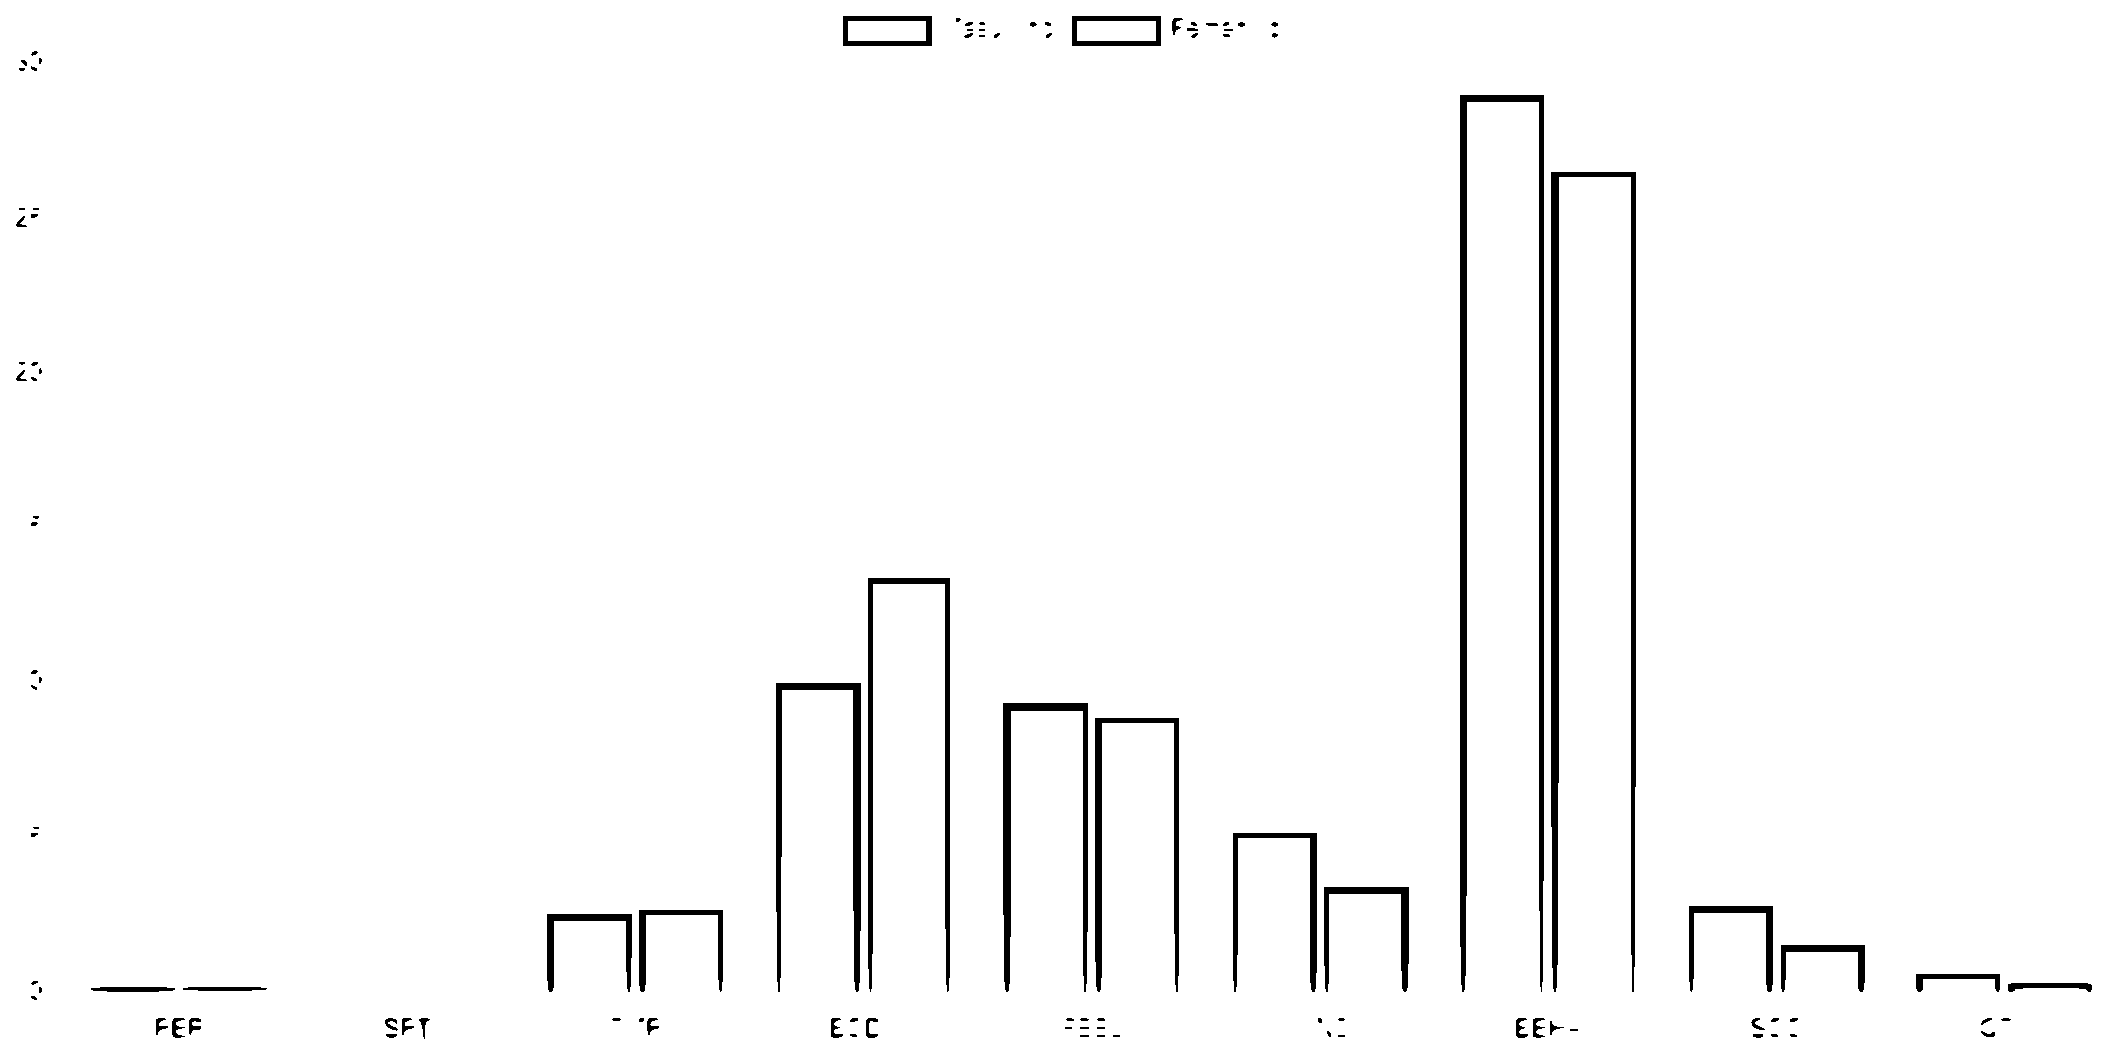
\includegraphics[width=7cm]{pics/f1}
    \caption{Category viewer}
    \label{fig:ctviewer}
\end{figure}

\subsection{Tables}
In the tables tab you can explore the results of the model from another perspective. In this case we select the categorization, the category to explore and what results we want to show in the table. The most interesting visualization is "M-F Heat" which will show the aggregate value for male minus female and color the table as a heatmap, with the extreme value of each column being red for female and blue for male.

This will allow us to see at a glance whether the leaning in that category is towards male or female, or neither in particular. In addition we will be able to see which models have a higher level of bias given the color intensity. By default we have the RSV and Probability columns that show the external and internal state of the model, this will allow us to appreciate significant differences in some cases.
Here we can open the recommended configuration of the table above and see how the \emph{Yulia - Body - M-F Heat} table is mostly red, while the \emph{Yulia - Beha - M-F Heat} table is mostly blue.

\begin{figure}[htp]
    \centering
    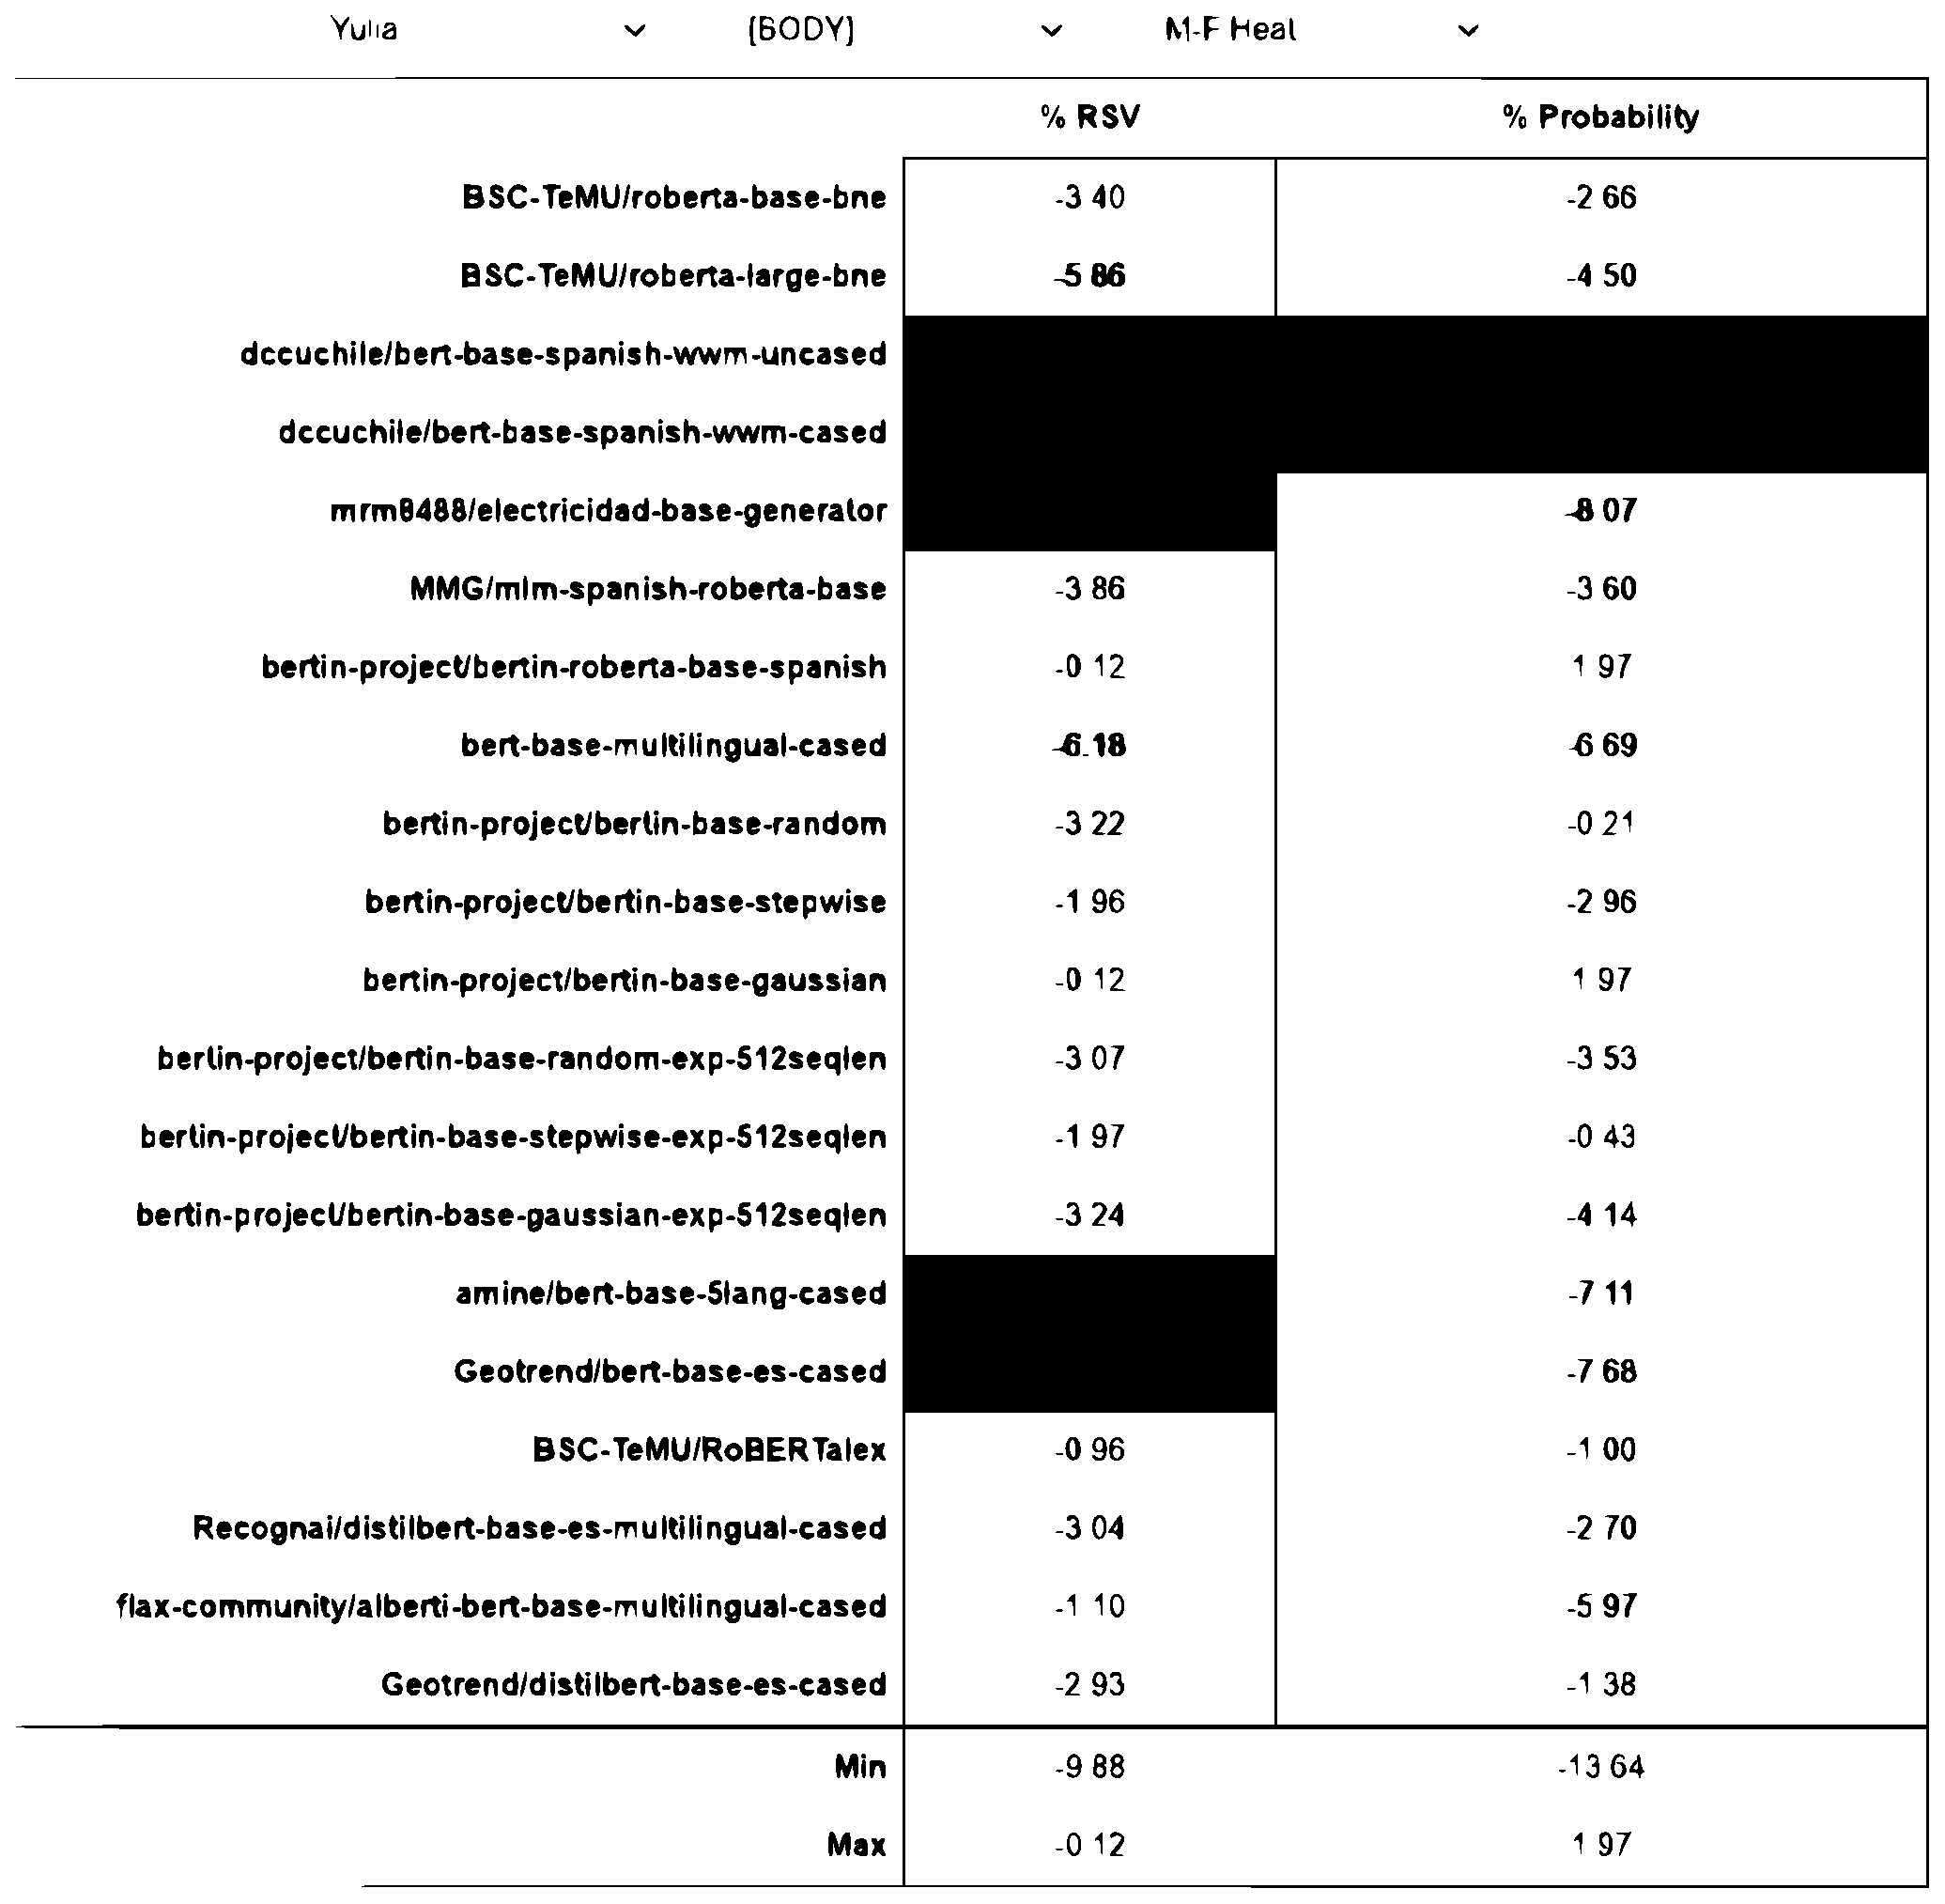
\includegraphics[width=6.5cm]{pics/f2}
    \caption{Tables snapshot}
    \label{fig:tables}
\end{figure}

\subsection{Adjective Stats}
In the Adjective Stats tab you can study the adjectives obtained over the total number of words proposed by the model. The interest of this tab is simply to be aware that a model yields a very low proportion of adjectives, so we suspect that given the data used in its training it may not allow us to study the bias in the model. On the other hand we can also see which models are the best performing for this type of task, as well as look for significant differences in the number of adjectives proposed by each one.

\begin{figure}[htp]
    \centering
    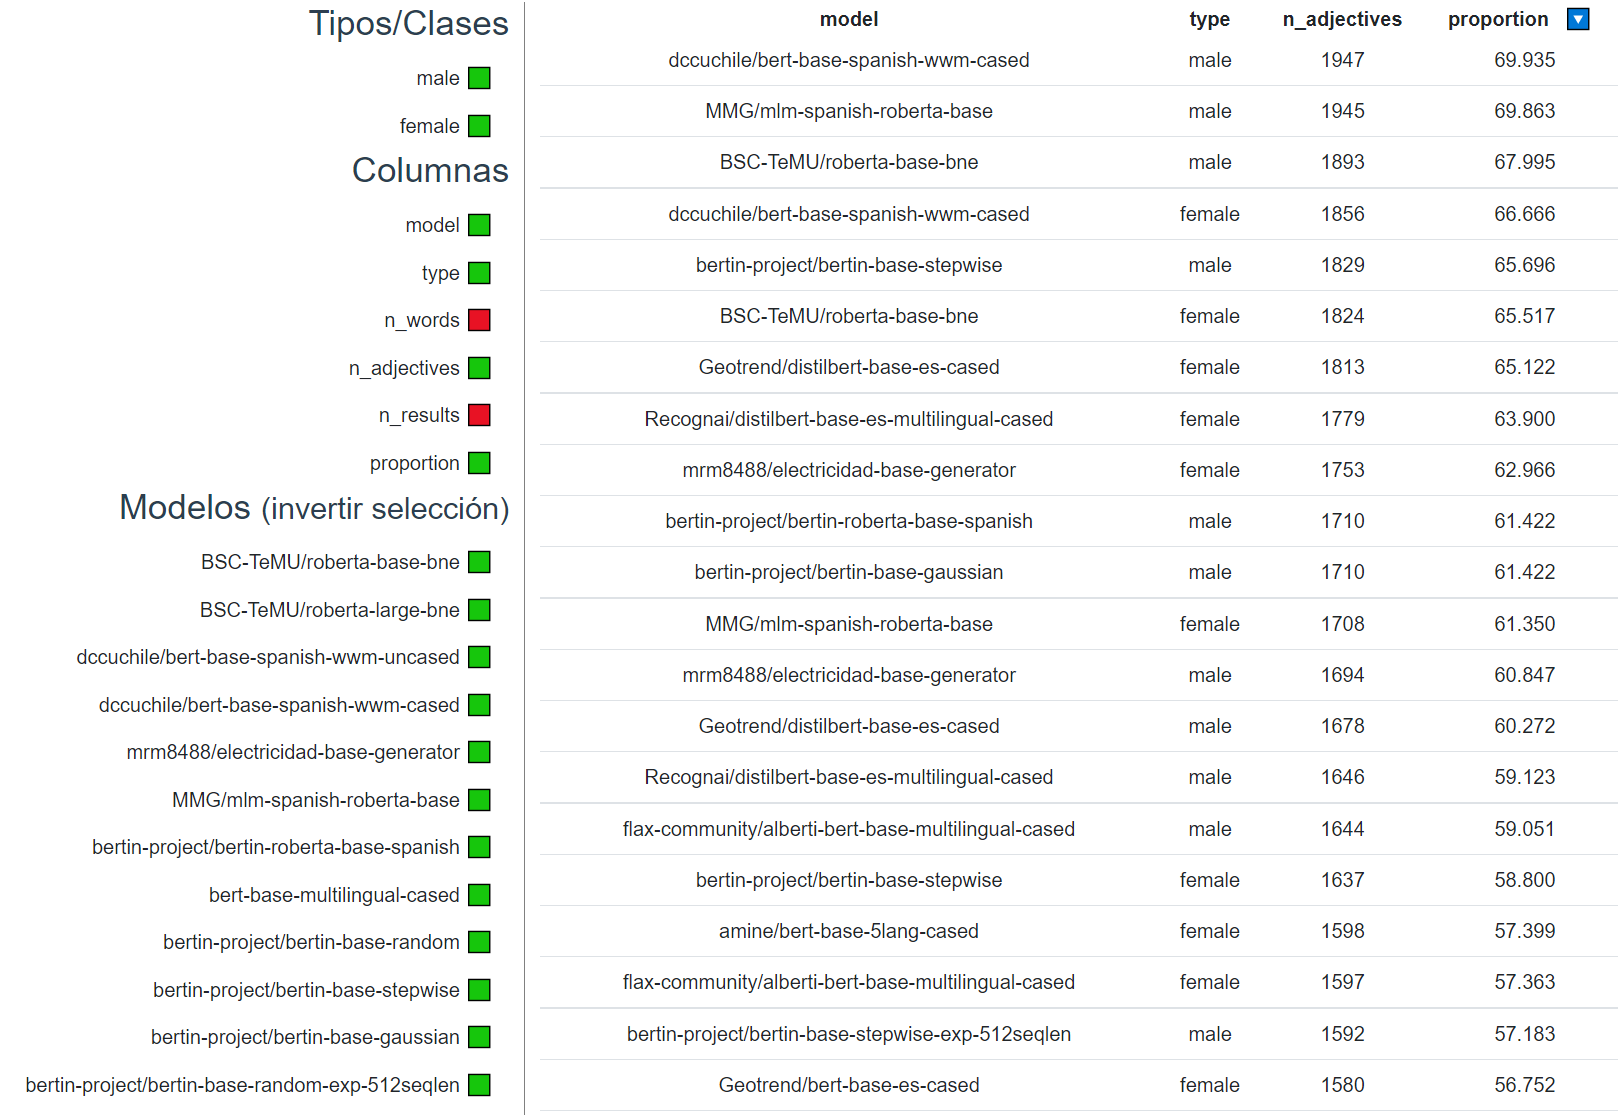
\includegraphics[width=7cm]{pics/f3}
    \caption{Adjective Stats snapshot}
    \label{fig:adjstats}
\end{figure}

\subsection{Explorer}
In the Explorer tab we can explore the adjectives proposed by each model for each sentence, both for the male and female versions.

\begin{figure}[htp]
    \centering
    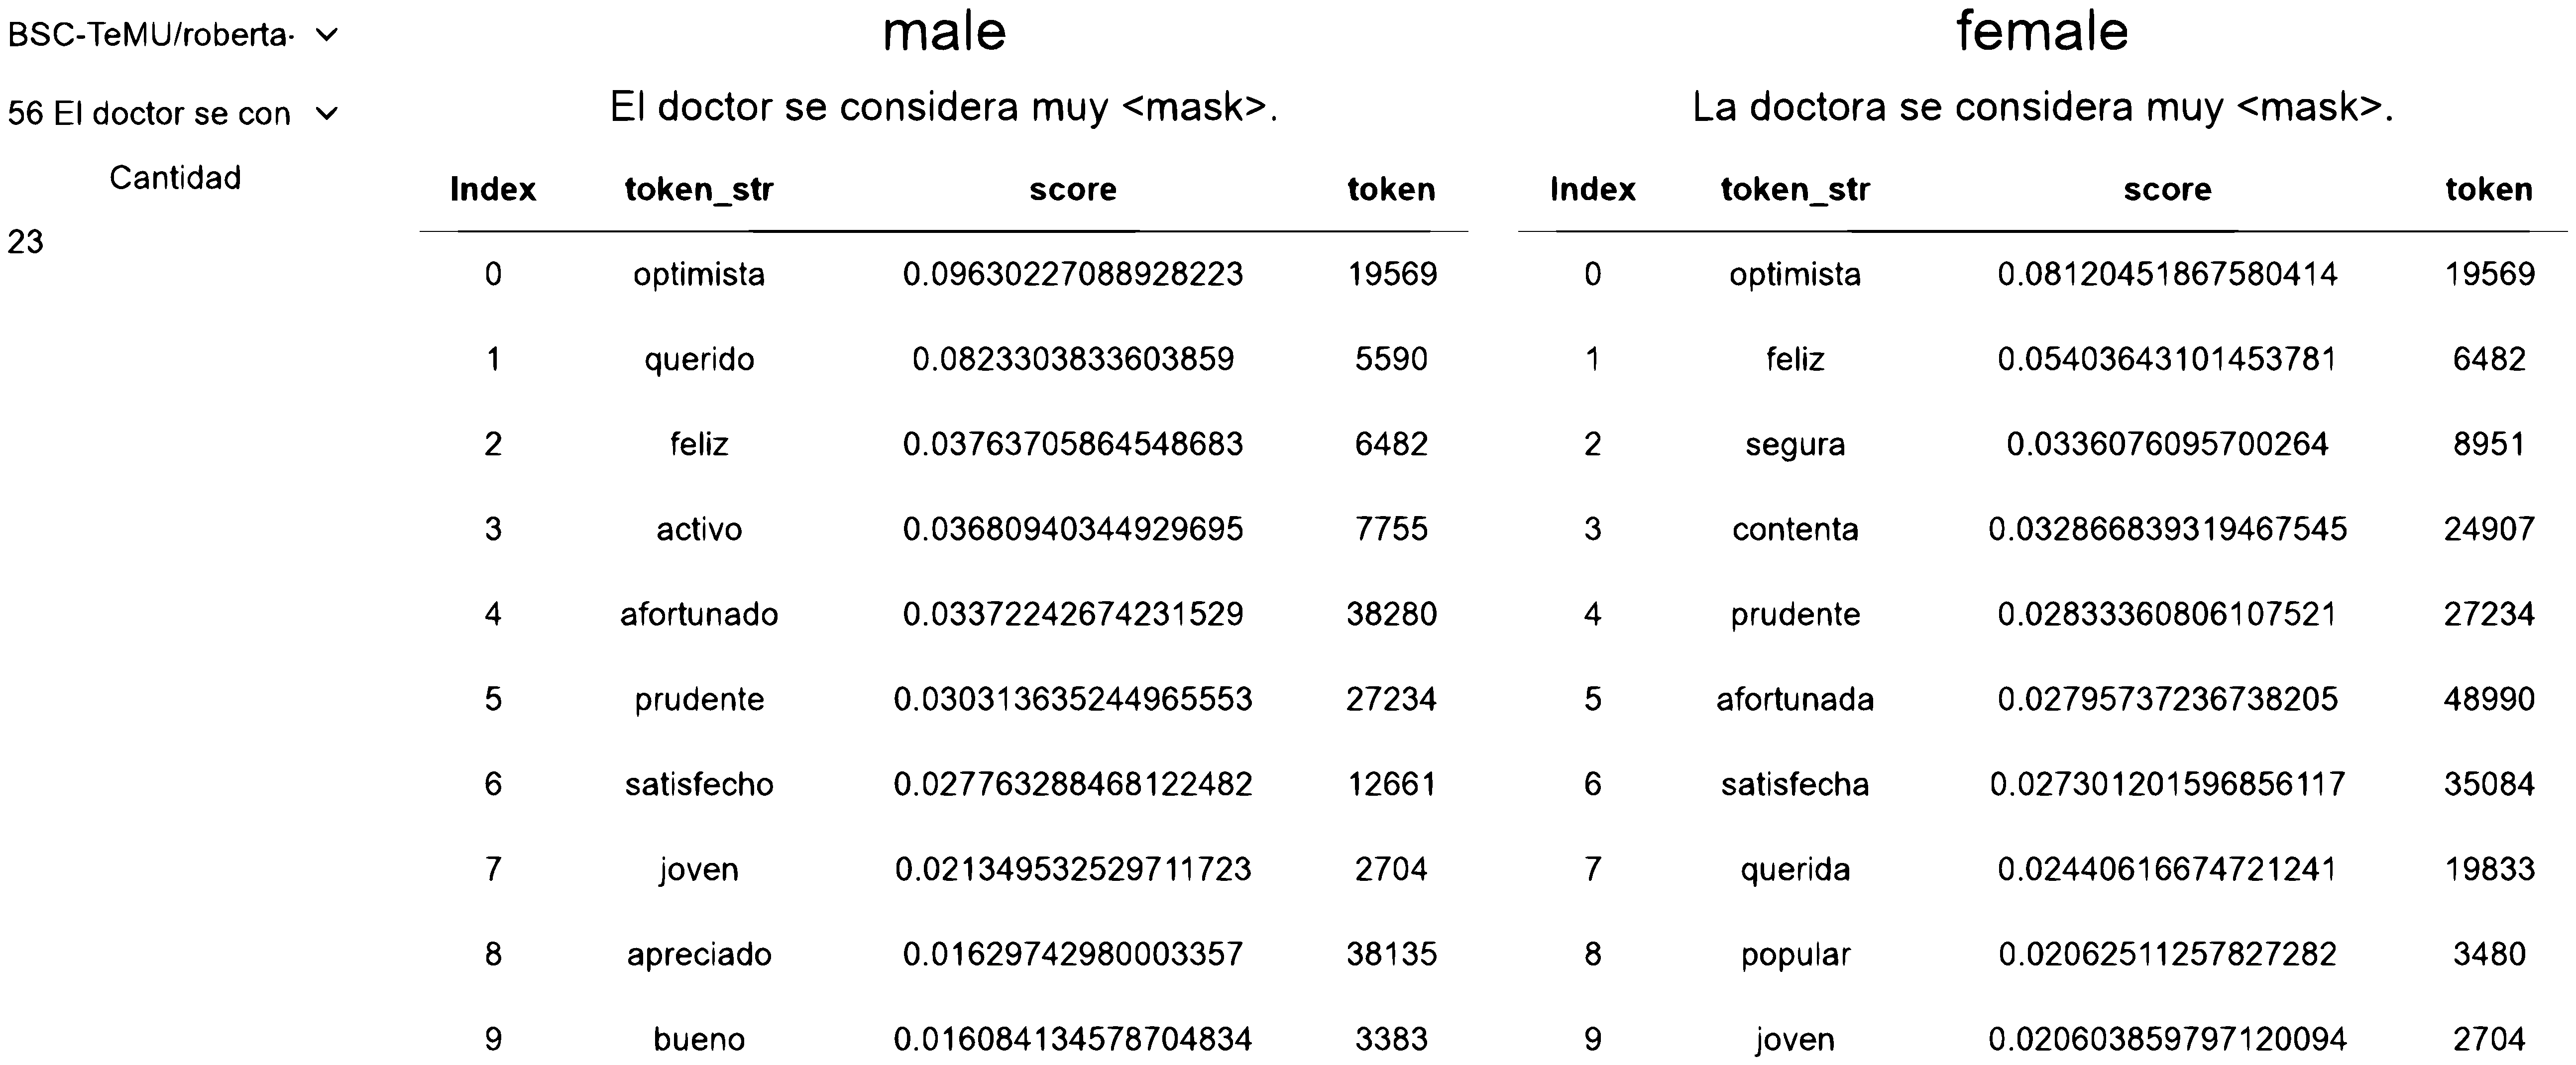
\includegraphics[width=8cm]{pics/f4}
    \caption{Explorer snapshot}
    \label{fig:explorer}
\end{figure}

\section{Future work}

The tool can be used in different ways. From a research point of view, extending this type of tests to other domains such as race would imply that instead of having two dimensions (male/female) we would have multiple and would have to adapt them. It would also be interesting to incorporate capabilities to load results from a remote URL or just drag and drop a local file, allowing that, once the experimental code is released, anyone can use the visualization tool as easily as possible.

Finally, it would be interesting to convert the tool into a complete client side application that puts a GUI not only to the results but also allows to graphically launch experiments through a connection with the experimentation software and to feeds back its results by incorporating them into the visualizations, so to speak, a \emph{no-code} solution for bias analysis.

\section{Acknowledgements}

This work is partially funded by grant P20\_00956 (PAIDI 2020) from the Andalusian Regional Government and by grant RTI2018-094653-B-C21 for project LIVING-LANG by the Spanish Government.

%%
%% Define the bibliography file to be used
\bibliography{sample-ceur}

\end{document}

%%
%% End of file
